{\setlength{\chapterfontsize}{23pt}
\chapter{Web service implementations}
}

\section{Data structures}
In this section, we describe the data structures used in our implementation. We cover the data contained in LameDuck and NiceView, followed by the more advanced BPEL and REST implementations.

\subsection{LameDuck}
LameDuck implement the data as described in the project description. To store this, we save all Flight Information both as lists of Flight Informations with the same origin airport and store a link from the Booking Number to the matching Flight Information. This is done to make lookups easier to perform. It does add some extra bookkeeping at initialization of the data. The overall data structure is shown in Fig.~\ref{fig:lameduck_class}

\begin{figure}[H]
\centering
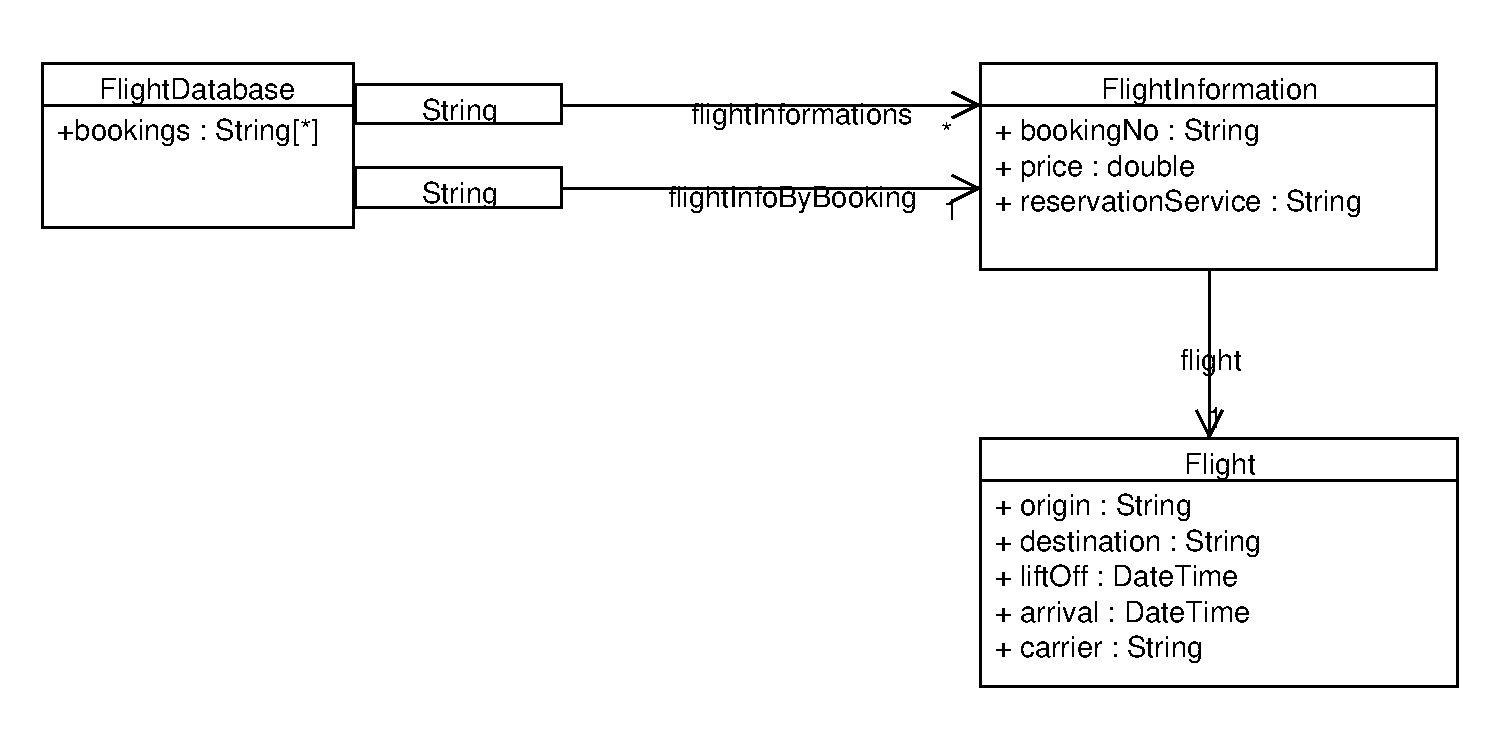
\includegraphics[width=0.8\textwidth]{LameDuckClass}
\caption{Datamodel of LameDuck}
\label{fig:lameduck_class}
\end{figure}

\subsection{NiceView}
\todo{NiceView klasse diagram}
\subsection{TravelGood - BPEL}
\todo{BPEL klasse diagram}

\subsection{TravelGood - RESTful}
\todo{REST klasse diagram}
\section{Airline- and hotel services}
Both LameDuck and NiceView are implemented using RPC-Literal style. This has been done for the simplicity of the format, while we sacrifice things from the document style binding, such as reduced overhead in the SOAP message as well as the ability to validate the SOAP message. We simply assume that the messages are formatted correctly.
Also, following the rationale from \cite{papazoglou2008web}, we this implementation is a synchronous service with parameter passing rather than an asynchronous document passing service.
\todo{Vi bør have en bedre grund til at vi ikke bruger Document style. Er denne ok? (KRC)}

For both services, we have developed a small suite of unit tests, that can be used to ensure that both services are running, before running tests for the BPEL/RESTful implementations. For this purpose, we have added a service along with the required one, to reset the databases of both services. To this end, the databases has been implemented using the singleton pattern, so both service classes works on the same database.


\subsection{LameDuck}
The LameDuck service has been implemented with a wrapper class that implements the web service related things. The actual data is stored in a hard coded database, which is initialized by the web service class. This way we separate the business logic of communicating with the world from the business logic of maintaining the flights and the bookings. The web service class is also responsible for communicating with the bank when necessary, separating handling of money from handling flights.

We have created some hardcoded test data, which can be reset using a separate web service, that should only be used during testing. As such this web service is implemented with a separate wsdl. To allow both services to access the database, it has been implemented as a singleton object.


\subsection{NiceView}
The NiceView service has been implemented similarly to that of our LameDuck service, just with hotels instead of flights.

It also has a separate reset service from which one can reset our database to the initial state.


